%frog manual rev 0.1
\documentclass{book}

\usepackage{epsf}
\usepackage{epsfig}
\usepackage{a4wide}
\usepackage{palatino}
\usepackage{fullname}
\usepackage{url}
\usepackage[utf8]{inputenc}
\usepackage{amsmath}
\usepackage{graphicx}
\usepackage{multicol,lipsum}
\usepackage[bottom=2cm,top=2cm,left=2cm,right=2cm]{geometry}
\usepackage{covington}
% * <iris@i-hx.nl> 2016-01-29T14:32:44.513Z:
% timbl manual is : https://www.overleaf.com/1292125vnpfbk
% ^.

\begin{document}
%\maketitle

\begin{titlepage}
	\begin{center}


        \vspace{115pt}
        \textbf{\huge{Frog}
        \ \\
        \vspace{30pt}
        \Large{A Natural Language Processing Suite for Dutch
}}\\ %proycon: ik vind de titel een beetje lang en chaotisch, is 'NLP suite' niet  netter?
        \vspace{95pt}
        \textbf{\Large{Version 0.13.1 - FIRST DRAFT REVISION! NOT FINAL!}}\\  %proycon: Beschreven frog versie - revisie versie van documentatie
		\vspace{3,5cm}
        Iris Hendrickx, Antal van den Bosch, Maarten van Gompel, Ko van der Sloot and Walter Daelemans\\ %we kunnen de volgorde nog aanpassen hoor!
       Centre for Language Studies and Centre for Speech and Language Technology, Radboud University\\
       CLST Technical Report 16-02\\
     % Welk nr hebben we voor tech report?

	\end{center}

	\vspace{1cm}

	\begin{center}
		\vspace{\fill}
         June 2016
    \end{center}
\end{titlepage}
%%\newpage
\tableofcontents
\thispagestyle{empty}

\newpage
\pagenumbering{arabic}

% % % % % % % % % % % % % % % % % % % % % % % % % % %

%(proycon) Omdat overleaf blijkbaar de git history niet synchroniseert met de versie
%labels, gooi ik de git history hier als commentaar zodat we een beetje zicht
%hebben op wat er gebeurd is:

%2016-03-23 08:30 Iris Hendrickx      o [master] {origin/master} {origin/HEAD} Update on Overleaf.
%2016-03-15 09:48 Iris Hendrickx      o saving some intermediate version
%2016-03-09 16:54 Iris Hendrickx      o Update on Overleaf.
%2016-03-09 14:56 Iris Hendrickx      o Update on Overleaf.
%2016-03-08 09:56 Anonymous           o Update on Overleaf
%2016-03-08 10:56 Maarten van Gompel  o minor fix
%2016-03-08 10:49 Maarten van Gompel  o added FrogOptions in python section
%2016-03-08 10:44 Maarten van Gompel  o ChangeLog
%2016-03-08 10:43 Maarten van Gompel  o Wrote "Using Frog from Python" section
%2016-03-08 10:15 Maarten van Gompel  o moved Using Frog from Python
%2016-03-08 10:14 Maarten van Gompel  o minor fix
%2016-03-08 09:56 Maarten van Gompel  o minor edits in NER section
%2016-03-07 23:41 Mustafa Erkan Basar o Update on Overleaf.
%2016-03-07 20:46 Maarten van Gompel  o added Server mode section
%2016-03-07 20:17 Maarten van Gompel  o ChangeLog
%2016-03-07 20:12 Maarten van Gompel o minor changes
%2016-03-07 20:08 Maarten van Gompel o minor changes
%2016-03-07 20:03 Maarten van Gompel o added references to frogr and gorf in credit section + link to github issue tracker
%2016-03-07 19:59 Maarten van Gompel o added Machiel Molenaar and his Go client in the credits
%2016-03-07 19:57 Maarten van Gompel o removed "please cite" in license, mentioned later already
%2016-03-07 19:53 Maarten van Gompel o retitled "Example usage of Frog" to "Frog in practice"
%2016-03-07 19:52 Maarten van Gompel o structure update
%2016-03-07 19:47 Maarten van Gompel o edited MWU section
%2016-03-07 19:41 Maarten van Gompel o edited encoding and tokenizer sections
%2016-03-07 19:37 Maarten van Gompel o interactive mode
%2016-03-07 19:32 Maarten van Gompel o User guide edits
%2016-03-07 19:05 Maarten van Gompel o editing quick start guide
%2016-03-07 18:42 Maarten van Gompel M─┐ Merge branch 'master' of https://git.overleaf.com/4159303gcfrtm
%2016-03-07 17:22 Anonymous          │ o Update on Overleaf.
%2016-03-07 18:41 Maarten van Gompel o │ installation instructions
%2016-03-07 18:29 Maarten van Gompel o │ syntax
%2016-03-07 18:21 Maarten van Gompel M─┘ Merge branch 'master' of https://git.overleaf.com/4159303gcfrtm
%2016-03-07 17:00 antalvdb           │ o Update on Overleaf.
%2016-03-07 18:20 Maarten van Gompel o │ edited installation section
%2016-03-07 17:43 Maarten van Gompel o─┘ edited license section (explicit reference to GPL v3)
%2016-03-07 17:42 Maarten van Gompel o Edited introduction (Frog in 150 words)
%2016-03-07 17:34 Maarten van Gompel o added Frog version - documentation revision
%2016-03-07 17:29 Maarten van Gompel o LaTeX source cleanup, no actual content changes yet
%2016-03-03 13:44 Iris Hendrickx     o Update on Overleaf.
%2016-03-03 13:40 Maarten van Gompel I first shared version iris


% % % % % % % % % % % % % % % % % % % % % % % % % % %


%todo
% -toevoegen tabel met alle commandline options
% - alle config opties in H5 zetten, plus de standaard frog config als een voorbeeld. : char_filter_file  gebruikt in: mbma, mblem en de PoS tagger
\chapter{Introduction}

Frog is an integration of memory-based natural language processing (NLP)
modules developed for Dutch. Frog performs tokenization, part-of-speech tagging,
lemmatization and morphological segmentation of word tokens. At the sentence
level Frog identifies non-embedded phrase chunks in the sentence, recognizes named
entities and assigns a dependency parse graph. Frog produces output in either FoLiA XML
or a simple tab-delimited column format with one token per line. All
NLP modules are based on Timbl, the Tilburg memory-based learning software
package. Most modules were created in the 1990s at the ILK Research Group
(Tilburg University, the Netherlands) and the CLiPS Research Centre (University
of Antwerp, Belgium). Over the years they have been integrated into a single
text processing tool, which is currently maintained and developed by the
Language Machines Research Group and the Centre for Language and Speech
Technology at Radboud University (Nijmegen, the Netherlands).

\chapter{License}

Frog is free and open software. You can redistribute it and/or modify it under
the terms of the GNU General Public License v3 as published by the Free Software
Foundation.  You should have received a copy of the GNU General Public License
along with Frog. If not, see \url{http://www.gnu.org/licenses/gpl.html}.

\chapter{Installation}

You can download Frog, manually compile and install it from source.  However,
due to the many dependencies and required technical expertise this is not an
easy endeavor.

Linux users should first check whether their distribution's package manager has
up-to-date packages for Frog, as this provides the easiest way of installation.

If no up-to-date package exists, we recommend to use \textbf{LaMachine}. Frog is
part of our LaMachine software distribution and includes all
necessary dependencies. It runs on Linux, BSD and Mac OS X. It can also run as
a virtual machine under other operating systems, including Windows.  LaMachine
makes the installation of Frog straightforward; detailed instructions for
the installation of LaMachine can be found here: \url{http://proycon.github.io/LaMachine/}.

\section{Manual compilation \& installation}

The source code of Frog for manual installation can be obtained from Github.
Because of file sizes and to cleanly separate code from data, the data and
configuration files for the modules of Frog have been packaged separately.

\begin{itemize}
    \item   Source code repository: \url{https://github.com/LanguageMachines/frog/}
    %iris: iets met stable release, wat is verschil?
    %proycon: verwerkt:
    \item   Stable releases\footnote{The source code repository points to the latest
            development version by default, which may contain experimental
            features. Stable releases are deliberate snapshots of the source
            code. It is recommended to grab the latest stable release.}:
            \url{https://github.com/LanguageMachines/frog/releases/}
    \item   Frog data repository: \url{https://github.com/LanguageMachines/frogdata/} (required dependency!)
\end{itemize}

To compile these manually, you first need current versions of the following
dependencies of our software, and compile and install them in the order
specified here:

\begin{itemize}
    \item \texttt{ticcutils}\footnote{\url{https://github.com/LanguageMachines/ticcutils}} - A shared utility library
    \item \texttt{libfolia}\footnote{\url{https://github.com/LanguageMachines/libfolia}}- A library for the FoLiA format
    \item \texttt{ucto}\footnote{\url{https://languagemachines.github.io/ucto}} - A rule-based tokenizer
    \item \texttt{timbl}\footnote{\url{https://languagemachines.github.io/timbl}} - The memory-based classifier engine
    \item \texttt{timblserver}\footnote{\url{https://github.com/LanguageMachines/timblserver}} - For server functionality around Timbl
    \item \texttt{mbt}\footnote{\url{https://languagemachines.github.io/mbt}}  - The memory-based tagger
\end{itemize}

You will also need the following 3rd party dependencies:

\begin{itemize}
    \item \textbf{icu} - A C++ library for Unicode and Globalization support.
        On Debian/Ubuntu systems, install the package \texttt{libicu-dev}.
    \item \textbf{libxml2} - An XML library. On Debian/Ubuntu systems install
        the package \texttt{libxml2-dev}.
    \item A sane build environment with a C++ compiler (e.g.\ gcc or clang), autotools, autoconf-archive, libtool, pkg-config
\end{itemize}

The actual compilation proceeds by entering the Frog directory and issuing the following
commands:

\begin{verbatim}
$ bash bootstrap.sh
$ ./configure
$ make
$ sudo make install
\end{verbatim}

To install in a non-standard location (\texttt{/usr/local/} by default), you
may use \\ the \texttt{--prefix=/desired/installation/path/} option.

\chapter{User guide}
\label{ch-uguide}

Frog aims to automatically enrich Dutch text with linguistic information of various forms.
Frog integrates several NLP modules that perform the following tasks: tokenize
text to split punctuation from word forms (including recognition of sentence boundaries and
multi-word units), assignment of part-of-speech tags, lemmas, and morphological and
syntactic information to words.

In the next part we first give a brief explanation on running Frog to get you
started quickly, followed by a more elaborate description of using Frog and how
to manipulate the settings for each of the separate modules. In Chapter~
\ref{ch-bg} we discuss background information of Frog and the detailed
architecture of the modules.

\section{Quick start guide}

Frog is developed as a command line tool. We assume the reader already has at
least basic command line skills.

Typing {\tt frog -h} on the command
line results in a brief overview of all available command line options. Frog is
typically run on an input document, which is specified using the {\tt -t} option for
plain text documents, or {\tt -x} for documents in the FoLiA XML format. It is,
however, also possible to run it interactively or as a server.
%Ko: in feite is de -t optie (bijna?) nooit nodig
% frog test.txt werkt ook. Evenals frog *.txt
We show an example of the output of Frog when processing the contents of a
plain-text file \texttt{test.txt}, containing just the sentence {\it In '41 werd aan de stamkaart een
z.g.\ inlegvel toegevoegd.}

We run Frog as follows: {\tt \$ frog -t test.txt }

Frog will present the output as shown in example~\ref{ex-frog-out} below:

\begin{example}
\label{ex-frog-out}
\scalebox{0.8}{
\begin{tabular}{llllllllll}
\small
1 & 2 & 3 & 4 & 5 & 6 & 7 & 8 & 9 & 10\\
1 & In & in & [in] & VZ(init) & 0.987660 & O & B-PP & 0 & ROOT\\
2 & '41 & '41 & ['41] & TW(hoofd,vrij) & 0.719498 & O & B-NP & 1 & obj1\\
3 & werd & worden & [word] & WW(pv,verl,ev) & 0.999799 & O & B-VP & 0 & ROOT\\
4 & aan & aan & [aan] & VZ(init) & 0.996734 & O & B-PP & 10 & mod\\
5 & de & de & [de] & LID(bep,stan,rest) & 0.999964 & O & B-NP & 6 & det\\
6 & stamkaart & stamkaart & [stam][kaart] & N(soort,ev,basis,zijd,stan) & 0.996536 & O & I-NP & 4 &  obj1\\
7 & een & een & [een] & LID(onbep,stan,agr) & 0.995147 & O & B-NP & 9 & det\\
8 & z.g. & z.g. & [z.g.] & ADJ(prenom,basis,met-e,stan) & 0.500000 & O & I-NP & 9 & mod\\
9 & inlegvel & inlegvel & [in][leg][vel] & N(soort,ev,basis,zijd,stan) & 1.000000 & O &	I-NP & 10 &	obj1\\
10 & toegevoegd & toevoegen & [toe][ge][voeg][d] & WW(vd,vrij,zonder) & 0.998549 & O & 	B-VP & 3 & vc\\
11 & . & . & [.] & LET() & 1.000000 & O & O & 10 & punct\\
\end{tabular}
}
\end{example}

The ten TAB-delimited columns in the output of Frog contain the
information we list below. This columned output is intended for quick interpretation on
the terminal or in scripts. It does, however, not contain every detail available to Frog.

\begin{description}
    \item[1. Token number] (Number is reset every sentence.)
    \item[2. Token] The text of the token/word
    \item[3. Lemma] The lemma
    \item[4. Morphological segmentation] A morphological segmentation in which each morpheme is enclosed in square brackets
    \item[5. PoS tag] The Part-of-Speech tag according to the CGN tagset \cite{vanEynde2004}.
    \item[6. Confidence] in the PoS tag, a number between 0 and 1, representing
        the probability mass assigned to the best guess tag in the tag
        distribution
    \item[7. Named entity type] in BIO-encoding\footnote{B (begin) indicates the
            begin of the named entity, I (inside) indicates the continuation of a named
        entity, and O (outside) indicates that something is not a named entity}
    \item[8. Base phrase chunk] in BIO-encoding
    \item[9. Token number of head word] in dependency graph (according to the Frog parser)
    \item[10 Dependency relation type] of the word with head word
\end{description}


For full output, you will want to instruct Frog to output to a FoLiA XML file.
This is done using the {\tt -X} option, followed by the name of the output
file.

To run Frog in this way we execute: {\tt \$ frog -t test.txt -X test.xml}
The result is a file in FoLiA XML format \cite{FOLIAPAPER} that contains all
information in a more structured and verbose fashion. More information about
this file format, including a full specification, programming libraries, and
other tools, can be found on \url{https://proycon.github.io/folia}. We show an
example of the XML structure for the token {\it aangesneden} in example~\ref{ex-xml-tok}
and explain the details of this structure in section~\ref{sec-usage}. Each of these layers of linguistic output will be discussed in more detail in the next chapters.

\begin{example}
\label{ex-xml-tok}
\begin{verbatim}
<w xml:id="WP3452.p.1.s.1.w.4" class="WORD">
    <t>aangesneden</t>
    <pos class="WW(vd,vrij,zonder)" confidence="0.875" head="WW">
        <feat class="vd" subset="wvorm"/>
        <feat class="vrij" subset="positie"/>
        <feat class="zonder" subset="buiging"/>
    </pos>
    <lemma class="aansnijden"/>
    <morphology>
        <morpheme>
            <t>aan</t>
        </morpheme>
        <morpheme>
            <t>ge</t>
        </morpheme>
        <morpheme>
            <t>snijd</t>
        </morpheme>
        <morpheme>
            <t>en</t>
        </morpheme>
    </morphology>
</w>
\end{verbatim}
\end{example}

\subsubsection{Input and Output options}

By default the output of Frog is written to screen (i.e.\ standard output).
There are two options for outputting to file (which can also be called simultaneously):

\begin{itemize}
    \item \texttt{-o <filename>} -- Writes columned (TAB delimited) data to file.
    \item \texttt{-X <filename>} -- Writes FoLiA XML to file.
\end{itemize}

We already saw the input option {\tt -t <filename>} for plain-text files. It is
also possible to read FoLiA XML documents instead, using the {\tt -x
<filename>} option.

Besides input of a single plain text file, Frog also accepts a directory of
plain text files as input {\tt  --testdir=<directory> }, which can also be
written to an output directory with parameter {\tt --outputdir=<dir>}. The
FoLiA equivalent for {\tt --outputdir} is {\tt --xmldir}. To read multiple
FoLiA documents, instead of plain-text documents, from a directory, use {\tt -x
--testdir=<directory>}.


\subsection{Interactive Mode}

Frog can be started in an interactive mode by simply typing \texttt{frog} on the command
line. Frog will present a \texttt{frog>} prompt after which you can type text
for processing. By default, you will press ENTER at an empty prompt before Frog
will process the prior input. This allows for multiline sentences to be entered.
To change this behavior, you may want to start
Frog with the {\tt -n} option instead, which tells it to assume each input line
is a sentence. FoLiA input or output is not supported in interactive mode.

To exit this mode, type CTRL-D.

\subsection{Server mode}
\label{servermode}

Frog offers a server mode that launches it as a daemon to which multiple
clients can connect over TCP. The server mode is started using the \texttt{-S
<port>} option. Note that options like \texttt{-n} and \texttt{--skip} are valid in this mode too.

You can for example start a Frog server on port 12345 as follows: \texttt{\$ frog -S 12345}.

The simple protocol clients should adhere to is as follows:

\begin{itemize}
	\item The client sends text to process (may contain newlines)
	\item The client sends the string \texttt{EOT} followed by a newline
	\item The server responds with columned, TAB delimited output, one token per line, and an empty line between sentences.
    \item FoLiA input and output are also possible, using the \texttt{-x} and \texttt{-X} options without parameters. When \texttt{-X} is selected, TAB delimited output is suppressed.
    \item The last line of the server response consists of the string \texttt{READY}, so the client knows it received the full response.
\end{itemize}

Communicating with Frog on such a low-level may not be necessary, as there are
already some libraries available to communicate with Frog for several
programming languages:

\begin{itemize}
	\item Python -- \textbf{pynlpl.clients.frogclient}\footnote{\url{https://github.com/proycon/pynlpl}, supports both Python 2 and Python 3}
	\item R -- \textbf{frogr}\footnote{\url{https://github.com/vanatteveldt/frogr/}} -- by Wouter van Atteveldt
	\item Go -- \textbf{grof}\footnote{\url{https://github.com/Machiel/gorf}} -- by Machiel Molenaar
\end{itemize}

The following example shows how to communicate with the Frog server from Python
using the Frog client in PyNLPl, which can generally be installed with a simple
\texttt{pip install pynlpl}, or is already available if you use our LaMachine distribution.

\begin{verbatim}
from pynlpl.clients.frogclient import FrogClient

port = 12345
frogclient = FrogClient('localhost',port)

for data in frogclient.process("Dit is de tekst om te verwerken.")
  word, lemma, morph, pos = data[:4]
  #TODO: Further processing per word
\end{verbatim}

Do note that Python users may prefer using the \texttt{python-frog} binding
instead, which will be described in Section~\ref{pythonfrog}. This binds with Frog natively
without using a client/server model and therefore has better performance.


\section{Software usage}
\label{sec-usage}


\subsection{Character encoding}

Frog assumes the input text to be plain text in the UTF-8 character
encoding. However, Frog offers the option to specify another character encoding
as input with the option {\t t -e}. This options is passed on to the {\it Ucto} Tokenizer. It has some limitations, (see \ref{tokenizer}) and will be ignored when the Tokenizer is disabled. The character encodings are derived from
the ubiquitous unix tool {\it iconv } \footnote{In the current Frog version
UTF-16 is not accepted as input in Frog.}. The output of Frog will always be in
UTF-8 character encoding. Likewise, FoLiA XML defaults to UTF-8 as well.

%@Ko:
%cat bla
%Supermarkt Albert Heijn is tegenwoordig tot 's avonds laat open.
%En de rosé wijn met het zeeëgel logo is lekker.

%iconv -f utf-8 -t utf-16 < bla >bla-utf16
% frog -t bla-utf16 -e utf-16 -o bla.out
%geeft hele rare output in bla.out!

\subsection{Tokenizer}
\label{tokenizer}
%@Maarten kun je de Ucto bibtex aanvullen?
%proycon: done!

Frog uses the tokenization software {\it Ucto} \cite{UCTO} for sentence
boundary detection and to separate punctuation from words. In general,
recognizing sentence boundaries and punctuation is a simple task but
recognizing names and abbreviations is essential to perfom this task well. As
shown in example \ref{ex-frog-out}, the tokenizer recognizes abbreviations such
as {\tt z.g.} and {\tt `41} and considers them to be one token. Ucto uses
manually constructed rules and lists of Dutch names and abbreviations. Detailed
information on Ucto can be found on
\url{https://languagemachines.github.io/ucto/}.

The tokenizer module in Frog can be adjusted in several ways.  If the input
text is already split on sentence boundaries and has one sentence per line, the
{\tt -n} option can be used to prevent Frog from changing the existing sentence
boundaries. When sentence boundaries were already marked with a specific
marker, one can specify this marker as {\tt --uttmarker "marker"}. The marker
strings will be ignored and their positions will be taken as sentence
boundaries.

If the input text is already fully tokenized, the tokenization step in
Frog can be skipped altogether using the skip parameter {\tt --skip=t}.
\footnote{In fact the tokenizer still is used, but in \texttt{PassThru} mode. This allows for conversion to FoLiA XML and sentence detection.}
% iris: @Ko: werkt de -n optie ook op folia input?
% proycon: nee, dat is niet relevant, het concept van een 'input line' bestaat
% niet in FoLiA,

\subsection{Multi-word units}
\label{sec-mwu}

Frog recognizes certain special multi-word units (mwu) where a group of consecutive, related tokens is treated as one token. This behavior accommodates, and is in fact required for Frog's dependency parser as it is trained on a data set with such multi-word units. In the output the parts of the multi-word unit will be connected with an
underscore. The PoS-tag, morphological analysis, named entity label and chunk
label are concatenated in the same manner.

This multi-word detection can be disabled using the option {\tt
--skip=m}. When using this option, each element of the MWU is treated as
separate token. We shown an example sentence in \ref{ex_mwu} that has two multi-word units: {\it Albert Heijn } and {\it's avonds}. \\ \newline

\begin{tabular}{ll}
\label{ex_mwu}
\small
S: &Supermarkt Albert Heijn is tegenwoordig tot 's avonds laat open.\\
&\\
1 &	Supermarkt	supermarkt	[super][markt]	N(soort,ev,basis,zijd,stan)	0.542056	O	B-NP	3	su\\
2&	Albert\_Heijn	Albert\_Heijn	[Albert]\_[Heijn] SPEC(deeleigen)\_SPEC(deeleigen)	1.000000	B-ORG\_I-ORG	B-NP\_I-NP	1	app\\
3&	is	zijn	[zijn]	WW(pv,tgw,ev)	0.999150	O	B-VP	ROOT\\
4&	tegenwoordig	tegenwoordig	[tegenwoordig]	ADJ(vrij,basis,zonder)	0.994033	O	B-ADVP	3	predc\\
5&	tot	tot	[tot]	VZ(init)	0.964286	O	B-PP	None\\
6&	's\_avonds	's\_avond	['s]\_[avond][s]	LID(bep,gen,evmo)\_N(soort,ev,basis,gen)	0.962560	O\_O	O\_B-ADVP	5	obj1\\
7&	laat	laat	[laat]	ADJ(vrij,basis,zonder)	1.000000	O	B-VP	8	mod\\
8&	open	open	[open]	ADJ(vrij,basis,zonder)	0.983755	O	B-ADJP	3	predc\\
9&	.	.	[.]	LET()	1.000000	O	O	8	punct\\
\end{tabular}



\subsection{Lemmatizer}

The lemmatizer assigns the canonical form of a word to each word. For verbs
the canonical form is the infinitive, and for nouns it is the singular form.
The lemmatizer trained on the e-Lex lexicon \cite{e-lex}. It is dependent on
the Part-of-Speech tagger as it uses both the word form and the assigned PoS tag to
disambiguate between different candidate lemmas. For example the word {\it
zakken} used as a noun has the lemma {\it zak} while the verb has lemma {\it
zakken}.  Section \ref{sec-bg-lem} presents further details on the lemmatizer.


\subsection{Morphological Analyzer}

The morphological Analyzer (MBMA) cuts each word into its morphemes and shows the spelling changes that took place to create the word form. The fourth column in example \ref{ex-frog-out} shows the morphemes of the example sentence. MBMA  tries to decompose every token into morphemes, except for punctuation marks and names. Note that MBMA sometimes makes mistakes with unknown words such as abbreviations that are not included in the MBMA lexicon. The abbreviation {\tt z.g.} in the example is wrongly analyzed as consisting of two parts.
%iris: dit zou dus een verbeterpunt in MBMA kunnen zijn.
%ko: die fout maakt frog niet meer. (zie ook het aangehaalde voorbeedl 4.1 waar het WEL goed is)
As shown in the earlier XML example \ref{ex-xml-tok} the past particle {\it
aangesneden} is split into {\it[aan][ge][snijd][en]} where the morpheme {\it
[snijd]} is the root form of {\it sned}. More information about the MBMA
architecture can be found in \ref{sec-bg-morf}.


\subsection{Part-of-Speech Tagger}

The Part-of-Speech tagger uses the tag set of \emph{Corpus Gesproken Nederlands
(CNG)} \cite{vanEynde2004}. It has 12 main PoS tags (shown in table~\ref{tab-pos-tags})
and detailed features for type, gender, number, case, position, degree, and tense.

We show an example of the PoS tagger output in table~\ref{tab-pos-conf}. The tagger
also expresses how certain it was about its tag label in a confidence score
between 0 (not sure) and 1 (absolutely sure). In the example the PoS tagger is
very sure about the first four tokens but not about the label {\tt
N(soort,ev,basis,zijd,stan)} for the token {\it Psychologie} as it only has a
confidence score of 0.67. {\it Psychologie} is an ambiguous token and can also
be used as a name (tag SPEC).
%In the training set the token {\it Psychologie} occurs 23 times, 19 times as a
%name (label SPEC) and 4 times as noun (N).

%iris: willen we alle tags in detail beschrijven hier?
%The token 'Ik' is a pronoun (VNW), of the type nomimal(nom) personal(pers) first person(1) singular(ev) (pers,pron,nomin,vol,1,ev). The verb 'ben'

\begin{table}[h]
\begin{tabular}{ll}
ADJ & Adjective\\
BW & Adverb\\
LET & Punctuation\\
LID & Determiner\\
N & Noun\\
SPEC & Names and unknown\\
TSW & Interjection\\
TW & Numerator\\
VG & Conjunction\\
VNW & Pronoun\\
VZ & Preposition\\
WW & Verb\\
%  654059 &  ADJ & Adjective\\
% 1107840 & BW & Adverb\\
% 1008522 & LET & Punctuation\\
%  656629 & LID & Determiner\\
% 1188816 & N & Noun\\
%  334607 & SPEC & Names and unknown\\
%     872 & TSW & Interjection\\
%  141294 & TW & Numerator\\
%  635755 & VG & conjunction\\
% 1670448 & VNW & Pronoun\\
%  946779 & VZ & Preposition\\
% 1695812 & WW & Verb\\
\end{tabular}
\caption{\label{tab-pos-tags} The main tags in the CGN PoS-tag set.}
\end{table}


\begin{table}[h]
\begin{tabular}{llll}
34 &	Ik		&	VNW(pers,pron,nomin,vol,1,ev) &	0.999791\\
35 &	ben		&	WW(pv,tgw,ev) &	0.999589\\
36 &	ook		&	BW()&	0.999979\\
37 &	professor	&		N(soort,ev,basis,zijd,stan)	& 0.997691	\\
38 &	Psychologie	&		N(soort,ev,basis,zijd,stan) & {\bf 0.666667}\\
\end{tabular}
\caption{\label{tab-pos-conf} The PoS tagger assigns a confidence score to each tag.}
\end{table}

\subsection{Named Entity Recognition}
\label{sec-ner}

The Named Entity Recognizer (NER) detects names in the text and labels them as
location (\textsc{LOC}), person (\textsc{PER}), organization (\textsc{ORG}), product (\textsc{PRO}), event (\textsc{EVE}) or
miscellaneous (\textsc{MISC}).

%Events: Grammy awards, Second World War Product (Bible,New York Times)
Internally and in Frog's columned output, the tags use a so-called BIO paradigm where B stands for the beginning of the name, I signifies Inside the name, and O outside the name.

More detailed information about the NER module can be found in \ref{sec-bg-ner}.


\subsection{Phrase Chunker}
\label{sec-chunker}

The phrase chunker represents an intermediate step between part-of-speech tagging and full parsing as it produces a non-recursive, non-overlapping flat structure of recognized phrases in the text and classifies them with their grammatical function such as adverbial phrase (ADVP), verb phrase (VP) or noun phrase (NP). The tag labels produced by the chunker use the same type of BIO-tags (Beginning-Inside-Outside) as the named entity recognizer.
We show an example sentence in \ref{ex-chunk} where the four-word noun phrase {\it het cold case team} is recognized as one phrase. The prepositional phrases (PP) consist only of the preposition themselves due to the flat structure in which the relation between prepositions and noun phrases is not expressed (note that the dependency parse labels, section \ref{sec-dep} do express these relations). Here {\it Midden-Nederland} is recognized by the PoS tagger as name and therefor marked as a separate noun phrase that follows the noun phrase {\it de politie}.

\begin{example}
$[$Dat$]_{NP} [$bevestigt$]_{VP} [$het cold case team$]_{NP} [$van$]_{PP}] [$de politie$]_{NP} [$Midden-Nederland$]_{NP} [$ aan $]_{PP} [$de Telegraaf$]_{NP} [$ .
\end{example}

\begin{table}[h]
\begin{tabular}{lll}
1&Dat&B-NP\\
2&bevestigt&B-VP\\
3&het&B-NP\\
4&cold&I-NP\\
5&case&I-NP\\
6&team&I-NP\\
7&van&B-PP\\
8&de&B-NP\\
9&politie&I-NP\\
10&Midden-Nederland&B-NP\\
11&aan&B-PP\\
12&de&B-NP\\
13&Telegraaf&I-NP\\
14&.&O\\
\end{tabular}
\caption{\label{ex-chunk} The phrase chunker detects phrase boundaries and labels the phrases with their grammatical information.}
\end{table}



\subsection{Dependency Parser}
\label{sec-dep}

The Constraint-satisfaction inference-based dependency parser (CSI-DP) \cite{Canisius+2006} predicts grammatical relations between pairs of tokens. In each token pair relation, one token is the head and the other is the dependent. Together these relations represent the syntactic tree of the sentence. One token, usually the main verb in he sentence, forms the root of the tree and the other tokens depend on the root in a direct or indirect relation. CSI-DP is trained on the Alpino treebank \cite{Bouma+01} for Dutch and uses the Alpino syntactic labels listed in appendix \ref{app-dep}.
In the plain text output of Frog ( example \ref{ex-frog-out}) the dependency information is presented in the last two columns. The one-but-last column shows number of the token number of the head word of the dependency relation and the last column shows the grammatical relation type.
We show the last two columns of the CSI-DP output in table~\ref{ex-dep}.
The main verb {\it bevestigt} is root element of the sentence, the head of the
subject relation ({\tt su}) with the pronoun {\it Dat} and head in the object
relation ({\tt obj1}) with {\it team}. The noun {\it team} is the head in three
relations: the determiner({\tt det}) {\it het} and the two modifiers({\tt mod})
{\it cold case}. The name {\it Midden-Nederland} is linked as an apposition to
the noun {\it politie}. The prepositional phrase {\it van} is correctly
assigned to the head noun {\it team} but the phrase {\it aan} is mistakenly
linked to {\it politie} instead of the root verb {\it bevestigt}. Linking
prepositional phrases is a hard task for parsers \cite{atterer2007}. More
details on the architecture of the CSI-DP can be found in section~\ref{sec-bg-dep}
%M. Atterer and H. Sch¨utze. Prepositional phrase attachment
%without oracles. Computational Linguistics, 33(4):469–476,2007.
%M. Volk. How bad is the problem of PP-attachment? A comparison
%of English, German and Swedish. In Proceedings of the
%Third ACL-SIGSEM Workshop on Prepositions, pages 81–88,2006.
%J. Zavrel, W. Daelemans, and J. Veenstra. Resolving PP attachment
%ambiguities with memory-based learning. In Proceedings
%CoNLL 1997, pages 136–144, 1997.

\begin{table}[h]
\begin{tabular}{llll}
1&Dat&2&su\\
2&bevestigt&0&ROOT\\
3&het&6&det\\
4&cold&5&mod\\
5&case&6&mod\\
6&team&2&obj1\\
7&van&6&mod\\
8&de&9&det\\
9&politie&7&obj1\\
10&Midden-Nederland&9&app\\
11&aan&9&mod\\
12&de&13&det\\
13&Telegraaf&11&obj1\\
14&.&13&punct\\
\end{tabular}
\caption{\label{ex-dep} The dependency parser labels each token with a dependency relation to its head token and assigns the grammatical relation.}
\end{table}

\section{Using Frog from Python}
\label{pythonfrog}

It is possible to call Frog directly from Python using the \texttt{python-frog}
software library. Contrary to the Frog client for Python discussed in
Section~\ref{servermode}, this library is a direct binding with code from
Frog and does not use a client/server model. It therefore offers the tightest
form of integration, and highest performance, possible.

\subsection{Installation}

The Python-Frog library is not included with Frog itself, but is shipped
separately from \url{https://github.com/proycon/python-frog}.

Users who installed Frog using LaMachine, however, will already find that this software
has been installed.

Other users will need to compile and install it from
source. First ensure Frog itself is installed, then install the dependency
\texttt{cython}\footnote{Versions for Python 3 may be called \texttt{cython3}
on distributions such as Debian or Ubuntu}. Installation of Python-Frog is then
done by running: \texttt{\$ python setup.py install} from its directory.

\subsection{Usage}

The Python 3 example below illustrates how to parse text with Frog:

\begin{verbatim}
from frog import Frog, FrogOptions

frog = Frog(FrogOptions(parser=False))

output = frog.process_raw("Dit is een test")
print("RAW OUTPUT=",output)
output = frog.process("Dit is nog een test.")
print("PARSED OUTPUT=",output)
\end{verbatim}

To instantiate the \texttt{Frog} class, two arguments are needed. The first is a
\texttt{FrogOptions} instance that specifies the configuration options you want to
pass to Frog.

The \texttt{Frog} instance offers two methods: \texttt{process\_raw(text)} and
\texttt{process(text)}. The former just returns a string containing the usual
multiline, columned, and TAB delimiter output. The latter parses this string
into a dictionary. The example output of this from the script above is shown
below:

\begin{verbatim}
PARSED OUTPUT = [
 {'chunker': 'B-NP', 'index': '1', 'lemma': 'dit', 'ner': 'O',
  'pos': 'VNW(aanw,pron,stan,vol,3o,ev)', 'posprob': 0.777085, 'text': 'Dit', 'morph': '[dit]'},
 {'chunker': 'B-VP', 'index': '2', 'lemma': 'zijn', 'ner': 'O',
  'pos': 'WW(pv,tgw,ev)', 'posprob': 0.999966, 'text': 'is', 'morph': '[zijn]'},
 {'chunker': 'B-NP', 'index': '3', 'lemma': 'nog', 'ner': 'O',
  'pos': 'BW()', 'posprob': 0.99982, 'text': 'nog', 'morph': '[nog]'},
 {'chunker': 'I-NP', 'index': '4', 'lemma': 'een', 'ner': 'O',
  'pos': 'LID(onbep,stan,agr)', 'posprob': 0.995781, 'text': 'een', 'morph': '[een]'},
 {'chunker': 'I-NP', 'index': '5', 'lemma': 'test', 'ner': 'O',
  'pos': 'N(soort,ev,basis,zijd,stan)', 'posprob': 0.903055, 'text': 'test', 'morph': '[test]'},
 {'chunker': 'O', 'index': '6', 'eos': True, 'lemma': '.', 'ner': 'O',
  'pos': 'LET()', 'posprob': 1.0, 'text': '.', 'morph': '[.]'}
]
\end{verbatim}

There are various options you can set when creating an instance of \texttt{FrogOptions}, they are set as keyword arguments:

\begin{itemize}
	\item \texttt{tok} -- \emph{bool} -- Do tokenisation? (default: True)
	\item \texttt{lemma} -- \emph{bool} -- Do lemmatisation? (default: True)
	\item \texttt{morph} -- \emph{bool} -- Do morphological analysis? (default: True)
	\item \texttt{daringmorph} -- \emph{bool} -- Do morphological analysis in new experimental style? (default: False)
	\item \texttt{mwu} -- \emph{bool} -- Do Multi Word Unit detection? (default: True)
	\item \texttt{chunking} -- \emph{bool} -- Do Chunking/Shallow parsing? (default: True)
	\item \texttt{ner} -- \emph{bool} -- Do Named Entity Recognition? (default: True)
	\item \texttt{parser} -- \emph{bool} -- Do Dependency Parsing? (default: False).
	\item \texttt{xmlin} -- \emph{bool} -- Input is FoLiA XML (default: False)
	\item \texttt{xmlout} -- \emph{bool} -- Output is FoLiA XML (default: False)
	\item \texttt{docid} -- \emph{str} -- Document ID (for FoLiA)
	\item \texttt{numThreads} -- \emph{int} -- Number of threads to use (default: unset, unlimited)
\end{itemize}


\section{Frog generator}

Frog is developed for Dutch and intended as a ready tool to feed your text and to get detailed linguistic information as output.
However, it is possible to create a Frog lemmatizer and PoS-tagger for your own
data set, either for a specific Dutch corpus or for a corpus in a different language. {\tt Froggen} is a Frog-generator that expects as input a training corpus in a TAB separated column format of words, lemmas and PoS-tags.
%'Yo mam! Heb je de spekkoek al klaar? Coolio mam, echt vet lekker' Eh...watte? #kleinemannetjeswordengroot

This Dutch tweet annotated with lemma and PoS-tag information is an example of input required for {\tt froggen}:

\begin{verbatim}
Coolio coolio TSW
mam mam N
, , LET
echt echt ADJ
vet vet ADJ
lekker lekker ADJ
' ' LET
<utt>
Eh eh TSW
... ... LET
watte wat VNW
<utt>
? ? LET
#kleinemannetjeswordengroot #kleinemannetjeswordengroot HTAG
\end{verbatim}

Running {\tt froggen -T taggedcorpus -c my\_frog.cfg } will create a set of
Frog files, including the specified configuration file, that can be used to run
your own Frog. Your own instance of Frog should then be invoked using {\tt frog -c my\_frog.cfg}.

Besides the option to specify the Frog configuration file name to save the settings, one can also name the output directory where the frog files will be saved with {\tt [-O outputdir]}.
Froggen also allows an additional dictionary list of words, lemmas and PoS-tags
to improve the lemmatizer module with the option {\tt [-l lemmalist]}.
%(proycon): dat klinkt een beetje vaag, in welk formaat? is dat elders beschreven?


\chapter{Background}\label{ch-bg}
%for each module
% module architecture  classifier/rules, types of features
% training material
% evaluation results of module on benchmark data
% options to tune, retrain or replace module ?

%todo: geschiedenis vanaf mbsp en tadpole mbtalpa
\section{Once upon a time }
%iris: ik stem alvast voor de volgende naam voor de finale versie: Tadpole ->Frog -> Prince

The development of Frog's modules started in the nineties at the ILK Research Group
(Tilburg University, the Netherlands) and the CLiPS Research Centre (University
of Antwerp, Belgium). Most modules rely on Timbl, the Tilburg memory-based learning software
package \cite{timbl} or MBT the memory-based tagger-generator \cite{mbt}.
These modules were integrated into an NLP pipeline that was first named MB-TALPA and later Tadpole \cite{Tadpole}. Over the years, the modules were refined and retrained on larger data sets and the latest versions of each module are discussed in this chapter. We thank all programmers who worked on Frog and its predecessors in chapter \ref{ch-credit}.

The CliPS Research Centre also developed an English counterpart of Frog, a python module called MBSP (MBSP website: \url{http://www.clips.ua.ac.be/pages/MBSP}).
%Walter This is not actively supported anymore.

\section{Module overview}

Frog was developed as a modular system that allows for flexibility in usage.
In the current version of Frog, modules have a minimum of dependencies between each other so that the different modules can actually run in parallel processes, speeding up the performance time of Frog. The NER module, lemmatizer, phrase chunker and dependency parser are all independent from each other. All modules expect tokenized text as input. The lemmatizer, morphological analyzer and parser do depend on the PoS-tagger output.
These dependencies are depicted in figure \ref{fig-arch}. The tokenizer and multi-word chunker are rule-based modules while all other modules are based on trained memory-based classifiers.


\begin{figure*}[ht]
  \centering
   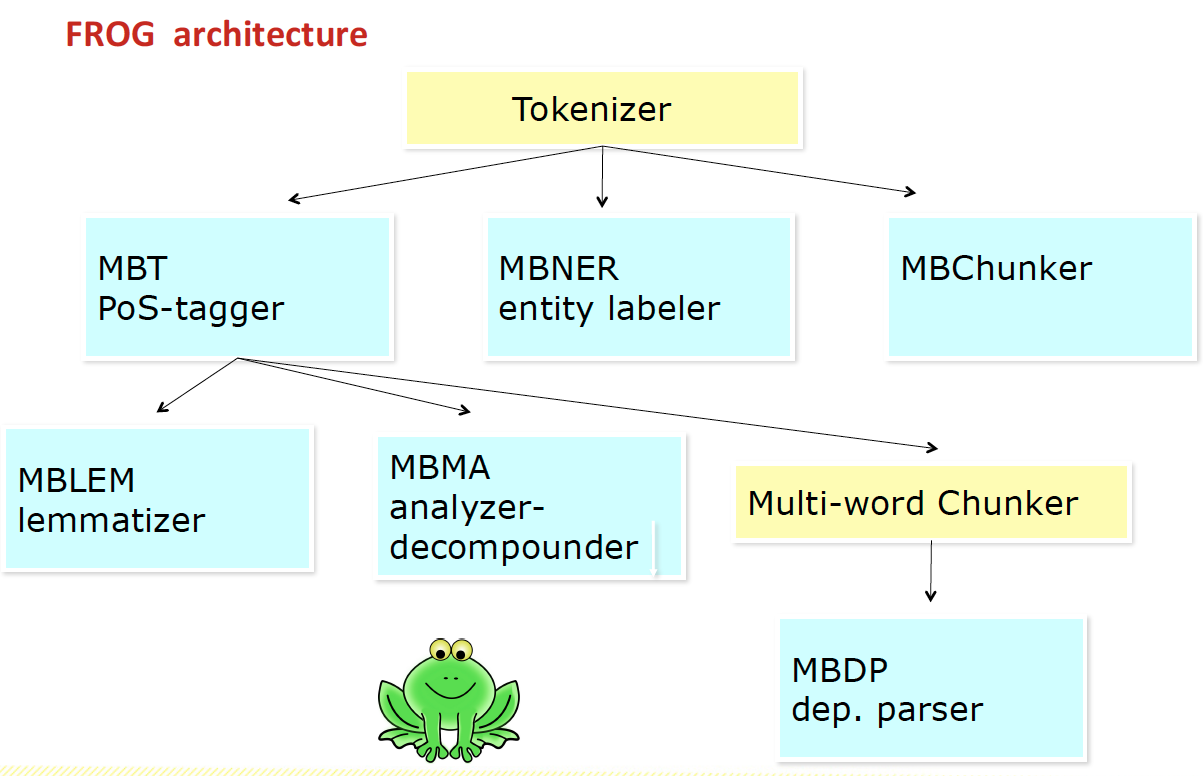
\includegraphics[scale=0.3]{frogarchitecture}
  \caption{Overview of the Frog architecture and the dependencies between the modules. All blue modules are based on memory-based learning while the yellow modules are rule-based.}
  \label{fig-arch}
\end{figure*}
%iris: picture taken from CLIN presentation.

\subsection{Configuration file}

For advanced usage of Frog, we can define the individual settings of each
module in the Frog configuration file ({\tt frog.cfg} in the frog source directory) or adapt some of the standard options. Editing this file requires detailed knowledge about the modules and relevant options will be discussed in the next sections. You can create your own frog configuration file and run frog with {\tt frog -c myconfigfile.cfg }.
%The configuration file also contains links to the Folia XML set definitions for the used XML tag sets.
The configuation file follows the INI file format\footnote{More about the INI file format:\url{https://en.wikipedia.org/wiki/INI_file)}} and is divided in individual sections for each of the modules. Some parts of the config file are obligatory and we show the
%De verschillende taggers staan in de configfile onder de kopjes:
%{\tt [[tagger]] }voor Nederlands de CGN tagger. (deze is min of meer verplicht)
%{\tt [[IOB]] } optioneel
%{\tt [[NER]] } optioneel

\begin{verbatim}
------------------------------------
[[tagger]]
set=http://ilk.uvt.nl/folia/sets/frog-mbpos-cgn
settings=morgen.settings

[[mblem]]
timblOpts=-a1 -w2 +vS
treeFile=morgen.tree

-------------------------------------
\end{verbatim}

There are some settings that each of the modules uses:

%1) settings=''' Wat verwijst naar een MBT settingsfile waarin de
%parameters staan waarmee de tagger getraind is.
%2) standaard opties:
\begin{itemize}
\item {\tt debug} Alternative to using {\tt --debug} on the command line. Debug values ranges from 1 (not very verbose) to 10??? (very verbose). Default setting is{\tt debug=0}. %@Ko levels?

\item {\tt version} module version that will be mentioned in FoLia XML output file.
%KO:in principe moet met elkeaanpassing in de MBMA trainingsdata dit aangepast,maar tot nu toe is dat nooit gedaan. Misschien aan beginnen als de MBMAdata stabiel genoeg is.

\item {\tt char\_filter\_file} file name of file where you can specify whether certain characters need to be replaced or ignored. For example, by default we translate all forms of exotic single quotes to the standard quote character.
%iris @KO har\_filter\_file="filename" en hoe moet dat file er dan uit zien, en kan ik dit idd aanpassen? bijv alles lower case maken? of alle nummers weggooien?

\item {\tt set} reference to the appropriate Folia XML set definition that is used in the module.
\end{itemize}










%@Maarten: deze file staat vol met verwijzingen naar niet-bestaande folia sets!
%http://ilk.uvt.nl/folia/sets/frog-depparse-nl
%en ook nog naar de oude ilk pagina.
%proycon: yep, klopt... Vrijwel alle sets bestaan nog niet, dat is op zich geen
%ramp, het fungeert vooral als een unieke ID, daarom kunnen we het eigenlijk
%ook niet zomaar wijzigen. Het was de bedoeling dat de oude ILK-pagina
%doorlinkt naar waar de sets wel staan als ze überhaupt bestaan. Maar dat is
%sindskort kapot zie ik, ik vraag het lars (systeembeheerder UvT) om te fixen.
%iris:oke Lars heeft het gefixed.

%proycon: hoort de configuration bij quick start? Ik zou het naar later verplaatsen
%iris: done.

\subsection{Tokenizer}
\label{sec-bg-tok}

The tokenizer Ucto has its own reference guide \cite{UCTO} and more detailed information can also be found on \url{https://languagemachines.github.io/ucto/}.


\subsection{Multi-word Units}

Extraction of multi-word units is a necessary pre-processing step for the Frog parser.
The mwu module is a simple script that takes as input the tokenized and PoS-tagged text and concatenates certain tokens like fixed expressions and names. Common mwu such as `ad hoc' are found with a dictionary lookup, and consecutive tokens that are labeled as `SPEC(deeleigen)' by the PoS-tagger are concatenated ({\tt gluetag} in the Frog config file).
The dictionary list of common mwu contains 1325 items and is distributed with the Frog source code and can be found under {\tt /etc/frog/Frog.mwu.1.0 }. These settings can be modified in the Frog config file.

%/vol/customopt/lamachine/etc/frog/Frog.mwu.1.0
%zo_optimaal_mogelijk BW_ADJ_ADJ
%verticale_diensten ADJ_N
%zommer_zonnewende
% iris: er is in Stevin ook een MWU lijst gemaakt. die is niet geheel bruikbaar want bevat ook vervoegde vormen 'geen hand voor ogen kunnen zien'
% maar goed, deze lijst is ook nogal arbitrair.

\subsection{Lemmatizer}
\label{sec-bg-lem}
%@kobus heeft jouw mblem.lex zelfde aantal items? 595,664? want dit geval komt nog van oude file.
% en hoeveel heeft mbma.lex?
The lemmatizer is trained on the e-Lex lexicon \cite{e-lex} with 595,664 unique word form - PoS-tag - lemma combinations. The e-Lex lexicon has been manually cleaned to correct several errors.
A timbl classifier is trained to learn the conversion of word forms to their lemmas. Each word form in the lexicon is represented as training instance consisting of the last 20 characters of the word form. Note that this abbreviates long words such as {\it consumptiemaatschappijen} to {\tt u m p t i e m a a t s c h a p p i j e n}.%{\it faculteitsvergaderingen} to {\tt u l t e i t s v e r g a d e r i n g e n}
In total, the training instance base has 402,734 unique word forms.
As in the Dutch language morphological changes occur in the word suffix,  leaving out the word beginning will not hinder the lemma assignment.
The class label of each instance is the PoStag and a rewrite rule to transform the word form to the lemma form. The rewrite rules are applied to the word form endings and delete or insert one or multiple characters. For example to get the lemma {\it bij} for the noun {\it bijen} we need to delete the ending {\it en} to derive the lemma.
We show some examples of instances in \ref{ex-lem} where the rewrite rules should be read as follows. For the example the word form {\it haarspleten} with label {\tt N(soort,mv,basis)+Dten+Iet} is a plural noun with lemma {\it haarspleet} that is derived by deleting(+D) the ending {\it ten} and inserting (+I) the new ending {\it et}.
For ambiguous word forms, the class label consists of multiple rewrite rules. The first rewrite rule with the same PoS tag is selected in such case.
Let's take as example the word {\it staken} that can be the plural noun form of {\it staak}, the present tense of the verb {\it staken} or the past tense of the verb {\it steken}. Here the PoS determines which rewrite rule is applied.
The lemmatizer does not take into account the sentence context of the words and in those rare cases where a word form has different lemmas associated with the same PoS-tags, a random choice is made.
%@antal: is de volgorde van de rewrite rules op  e-lex frequenties gebaseerd of random?
%Kobus, Maarten iemand zin om eens te kijken hoe vaak je onoplosbare gevallen hebt in het Nederlands? Daar ben ik echt best wel benieuwd naar!
%dus dezelfde POStag maar een andere rewrite rule.
%steengroeven  ->N(groeve)+Dn|N(groef)+Dven+If
%als ze heeeel zeldzaam zijn, dan hoeven we ze niet te noemen ?

\begin{example}
\label{ex-lem}

\scalebox{0.8}{
\begin{tabular}{ccccccccccccccl}
=&=&=&=&=&=&=&=&=&b&i&j&e&n&N(soort,mv,basis)+Den\\
=&=&=&h&a&a&r&s&p&l&e&t&e&n&N(soort,mv,basis)+Dten+Iet\\
=&=&=&=&h&a&a&r&s&t&u&k&j&e&N(soort,ev,dim,onz,stan)\\
=&=&=&=&=&=&=&=&s&t&a&k&e&n&N(soort,mv,basis)+Dken+Iak$|$WW(inf,nom,zonder,zonder-n)$|$WW(inf,prenom,zonder)$|$\\
 & && & & &&  & & & & & & &WW(inf,vrij,zonder)$|$WW(pv,tgw,mv)$|$WW(pv,verl,mv)+Daken+Ieken\\
=&=&=&=&=&=&=&s&p&l&e&t&e&n&N(soort,mv,basis)+Dten+Iet$|$WW(pv,verl,mv)+Deten+Iijten\\

\end{tabular}
}
\end{example}

%/vol/tensusers/ihendrickx/Data/frogdata/mblem.data:= = = = = = = = z w a l u w s t a a r t N(soort,ev,basis,zijd,stan)|WW(pv,tgw,ev)+Ien
%/vol/tensusers/ihendrickx/Data/frogdata/mblem.data:= = = = = = = v r i j d a g s t a a r t N(soort,ev,basis,zijd,stan)
% /vol/tensusers/ihendrickx/Data/frogdata/mblem.data:= = = = = = = = = = = = = = v u i l s t ADJ(nom,sup,zonder,zonder-n)+Dst|ADJ(prenom,sup,zonder)+Dst|ADJ(vrij,sup,zonder)+Dst
% = = = = = = = = s t e e n g r o e v e n N(16)+Dn|N(16)+Dven+If
%= = = = = = = = = = = = = = s t a a r t N(soort,ev,basis,zijd,stan)|WW(pv,tgw,ev)+Ien|WW(pv,tgw,met-t)+Dart+Iren

%wc /vol/bigdata/corpora/FrogData/mblem.data
%iris: zucht die datafile is helemaal verouderd en komt niet overeen met de werkelijkheid in Frog!
% dus Frog gebruikt niet langer mblem.translable (obsolete!) en de e-lex codes maar meteen gewoon de CGN tags.
%ko heeft me nu de nieuwe files gegeven zodat ik opniew kan tellen, en een paar voorbeeldjes eruit kan halen.
%done.
% /vol/tensusers/ihendrickx/Data/frogdata/


\subsection{Morphological Analyzer}
\label{sec-bg-morf}

The Morphological analyser MBMA \cite{MBMA} aims to decompose tokens into their morphemes reflecting possible spelling changes. Here we show two example words:
\begin{example}
\label{ex-longword}\begin{verbatim}
[leven][s][ver][zeker][ing][s][maatschappij][en]
[aan][deel][houd][er][s][vergader][ing][en]
\end{verbatim}
\end{example}
Internally, MBMA not only tries to split tokens into morphemes but also aims to classify each splitting point and its relation to the adjacent morpheme. MBMA is trained on the CELEX database \cite{Baayen+93}. Each word is represented by a set of instances that each represent one character of the word in context of 6 characters to the left and right. As example we show the 10 instances that were created for the word form {\it gesneden} in \ref{ex-mbma}. The general rule in Dutch to create a part particle of a verb is to add {\it ge-} at the beginning and add {\it -en} at the end. The first character 'g' is labeled with {\tt pv+Ige} indicating the start of an past particle (pv) where a prefix {\it ge} was inserted ({\tt +Ige)}. Instance 3 represents the actual start of the verb (V) and instance 5 reflects the spelling change that transforms the root form {\it snijd} to the actual used form {\it sned} ({\tt 0+Rij$>$e}: replace current character 'ij' with 'e' ). Instance 7 also has label 'pv' and denotes the end boundary of the root morpheme.

Timbl IGtree \cite{timbl} trained on 3179,331 instances extracted from that were based on the CELEX lexicon of 293,570 word forms. %wc laatste versie: /vol/tensusers/ihendrickx/Data/frogdata/mbma.data
 %oude versie /vol/bigdata/corpora/FrogData/mbma-merged.lex.back.151101 ??

The morphological character type classes result in a total 2708 class labels where the most frequent class '0' occurs in 69\% of the cases as most characters are inside an morpheme and to do not signify any morpheme border or spelling change.  %(2183976/3179357 = .686)
7\% of the instance represent a noun (N) starting point and 4\% a verb (V) starting point. The most frequent spelling changes are the insertion of an 'e' after the morpheme ({\tt 0/e}) (klopt dit?) or a plural inflection (denoted as 'm').

The MBMA module of Frog does not analyze every token in the text, it uses the PoS tags assigned by the PoS module to filter out punctuation and names (PoS 'SPEC') and words that we labeled as ABBREVIATION by the Tokeniser. For these cases, Frog keeps the token as it is without further analysis.

{\it Running frog with the parameter {\tt --deep-morph} results in a much richer morphological analysis including grammatical classes and spelling changes}.
%[[aan]preposition[ge]/participle/past-tense[snijd]verb[en]/participle/past-tense]verb

%  52459 m
%  85905 0/e
% 135803 V
% 221391 N
% 2183976 0

\begin{example}
\label{ex-mbma}
\begin{tabular}{lcccccccccccccl}
1 & \_&\_&\_&\_&\_&\_&{\bf g}&e&s&n&e&d&e&pv+Ige\\
2 & \_&\_&\_&\_&\_&g&e&s&n&e&d&e&n&0\\
3 & \_&\_&\_&\_&g&e&s&n&e&d&e&n&\_&V\\
4 & \_&\_&\_&g&e&s&n&e&d&e&n&\_&\_&0\\
5 & \_&\_&g&e&s&n&e&d&e&n&\_&\_&\_&0+Rij$>$e\\
6 &\_&g&e&s&n&e&d&e&n&\_&\_&\_&\_&0\\
7 & g&e&s&n&e&d&e&n&\_&\_&\_&\_&\_&pv\\
8 & e&s&n&e&d&e&n&\_&\_&\_&\_&\_&\_&0\\
\end{tabular}

\end{example}
%interessant dat de adjectieven geen morf analyse krijgen en verbs wel
% dus aangesneden/ADJ heeft als morf 'aangesneden' en als V wel [aan][ge][snijd][en]
%Ko: Inmiddels is dit gedrag veranderd denk ik.
%   aangesneden was in mbma alleen als WW bekend. %   Adjectivisch gebruik gaf een PoS tag mismatch en dan komt het originele woord als anaylyze er uit.
%   Nu "weet" mbma dat WW soms als ADJ optreden en geeft de WW analyze terug
% \begin{verbatim}
% _,_,_,_,_,a,f,g,e,z,o,n,k,0
% _,_,_,_,a,f,g,e,z,o,n,k,e,pv+Ige
% _,_,_,a,f,g,e,z,o,n,k,e,n,0
% _,_,a,f,g,e,z,o,n,k,e,n,_,V
% _,a,f,g,e,z,o,n,k,e,n,_,_,0+Ri>o
% a,f,g,e,z,o,n,k,e,n,_,_,_,0
% f,g,e,z,o,n,k,e,n,_,_,_,_,0
% g,e,z,o,n,k,e,n,_,_,_,_,_,pv
% e,z,o,n,k,e,n,_,_,_,_,_,_,0
% _,_,_,_,_,_,a,f,g,e,z,o,o,P
% --
% _,_,_,d,i,e,p,g,e,z,o,n,k,0
% _,_,d,i,e,p,g,e,z,o,n,k,e,A
% _,d,i,e,p,g,e,z,o,n,k,e,n,0
% d,i,e,p,g,e,z,o,n,k,e,n,_,0
% i,e,p,g,e,z,o,n,k,e,n,_,_,0
% e,p,g,e,z,o,n,k,e,n,_,_,_,0
% p,g,e,z,o,n,k,e,n,_,_,_,_,0
% g,e,z,o,n,k,e,n,_,_,_,_,_,0
% e,z,o,n,k,e,n,_,_,_,_,_,_,0/P
% _,_,_,_,_,_,d,i,e,p,g,i,n,A
% --
% e,z,o,n,g,e,n,_,_,_,_,_,_,0
% _,_,_,_,_,_,g,e,z,o,n,k,e,A|pv+Ige
% _,_,_,_,_,g,e,z,o,n,k,e,n,0
% _,_,_,_,g,e,z,o,n,k,e,n,_,0|V
% _,_,_,g,e,z,o,n,k,e,n,_,_,0|0+Ri>o
% _,_,g,e,z,o,n,k,e,n,_,_,_,0
% _,g,e,z,o,n,k,e,n,_,_,_,_,0
% g,e,z,o,n,k,e,n,_,_,_,_,_,0|pv
% e,z,o,n,k,e,n,_,_,_,_,_,_,0/P|0
% _,_,_,_,_,_,g,e,z,o,n,n,e,pv+Ige
% \end{verbatim}


%iris: NB in tadpole paper staat dat morf-analyzer 5 chars left en right heeft, en dus 11 features. Maar in huidige versie zijn dat er toch echt 13!
% en verder staat er dat het 363,690 woorden uit CELEX zijn en ik heb er nu slechts 293,570 ? groot verschil?
Note that the older version of the morphological analyzer reported in \cite{Tadpole} was trained on a slightly different version of the data with a context of only 5 instead of 6 characters left and right.
In that older study the performance of the morphological analyzer was evaluated on a 10\% held out set and an accuracy of 79\% on {\it unseen} words was attained.

\subsubsection{MBMA Configuration file options}
%Configuratie file opties:
When you want to set certain options for the MBMA module, place them under the heading {\tt [[mbma]] }in the Frog configuration file.

%iris: @Ko in hoeverre is het nuttig om config file opties te beschrijven als deze verplicht zijn en niet gewijzigd mogen of kunnen worden?
% ik beschrijf hierboven al dat MBMA op Celex is getraind.
% je kunt toch niet wijzigen: "clex-set=WOTAN" -> dan doet tie vast niks meer?

\begin{itemize}
\item {\tt set} FoLiA set name for the morphological tag set that MBMA uses.
\item {\tt clex-set} FoLiA set name PoS-tag- set that MBMA uses internally. As MBMA is trained on CELEX, it uses the CELEX POS-tag set, and not the default PoS-tag set (CGN tag set) of the Frog PoS tagger module. However, these internal pos-tags are mapped back to the CGN tag set.

%iris: @Ko wanneer precies gebruikt MBMA de CGN tag set en wanneer niet?
%NB:
%Daarnaast gebruikt MBMA ook de setnamen van de Tagger voor de PoS tags zoals die staan onder {\tt [[tagger]] }
%set-....


\item {\tt cgn\_clex\_main}File name of file that contains the mapping of CGN tags to
CELEX tags.
%iris @KO waar staat die file en hoe heet tie precies? En ik zie het nut niet heel erg van dit soort details in de Frog manual, is wel heeeel erg gedetaileerd.

%Ko:Die gebruikt MBMA dus bij de selectie van de 'juiste' analyze.

%\item {\tt cgn\_clex\_sub} De naam van de file met de (zeer beperkte!) mapping van
%CGN subtags naar MBMA. MBMA gebruikt die om gevonden inflecties te
%matchen aan CGN subtags. Voor verfijnde matching en desambiguering.

%\item {\tt filter\_diacritics} Hiermee zou je ervoor kunnen zorgen dat ALLE
%diacrieten uitgefilterd worden. waarmeer ideeën en ideeen intern
%hetzelfde woord zijn. Niet echt een goed plan. (misschien niet vermelden....?)




\item {\tt deep-morph} Alternative to using {\tt --deep-morph} on the command line.
\item {\tt treeFile}  Name of the trained MVMA Timbl tree (usually IG tree is used).
\item {\tt timbOpts}  Timbl options that were used for creating the MBMA treeFile.
\end{itemize}

\subsection{PoS Tagger}
\label{sec-bg-pos}

%/vol/bigdata/corpora/FrogData/cgn-wotan-dcoi.mbt
The PoS tagger in Frog is based on MBT, a memory-based tagger-generator and tagger\footnote{MBT available at http://languagemachines.github.io/mbt/}\cite{mbt} trained on a large Dutch corpus of 10,975,324 tokens in 933,891 sentences. This corpus is a mix of several manually annotated corpora but about 90\% of the data comes from the transcribed Spoken Dutch Corpus of about nine million tokens \cite{CGN2003}. The other ten precent of the training data comes from the ILK corpus (46K tokens), the D-Coi corpus (330K tokens) and the Eindhoven corpus (75K tokens) cite{uit den Boogaart 1975} that were re-tagged with CGN tag set.
%todo: citations toevoegen
The tag set consists of 12 coarse grained PoS-tags and 280 fine-grained PoS tag labels. Note that the chosen main categories (shown in table \ref{tab-pos-tags}) are well in line with a universal PoS tag set as proposed by \shortcite{Petrov2011} which has almost the same tags. The universal set has a {\it particles} tag for function words that signify negation, mood or tense while CGN has an  {\it interjection} tag to label words like `aha' and `ok\'e'  that are typically used in spoken utterances.

%Petrov: the following twelve POS tags:
%NOUN (nouns), VERB (verbs), ADJ (adjectives),
%ADV (adverbs), PRON (pronouns), DET (determiners
%and articles), ADP (prepositions and postpositions),
%NUM (numerals), CONJ (conjunctions), PRT
%(particles), ‘.’ (punctuation marks) and X (a catch-all
%for other categories such as abbreviations or foreign words).
%dit staat in Tadpole paper over tagger data:
% The data used for training the TADPOLE tagger consists of a broad selection
% of available manually annotated part-of-speech tagged corpora for Dutch tagged
% with the Spoken Dutch Corpus tagset (Van Eynde 2004): The approximately ninemillion
% word of the transcribed Spoken Dutch Corpus itself (Oostdijk, Goedertier,
% Van Eynde, Boves, Martens, Moortgat and Baayen 2002), the ILK corpus with
% approximately 46 thousand part-of-speech tagged words, the D-Coi corpus with
% approximately 330 thousand words, and the 754-thousandword Eindhoven corpus
% (Uit den Boogaart 1975) which has been automatically retagged with the Spoken
% Dutch Corpus tagset. Together this accounts for 10,979,827 manually-checked
% part-of-speech tagged words, all using the same rich tagset of 316 tags.

\subsection{Named Entity Recognition}\label{sec-bg-ner}

% module architecture  classifier/rules, types of features
% training material
% evaluation results of module on benchmark data
% options to tune, retrain or replace module ?


The Named Entity Recognizer (NER) is an MBT classifier \cite{mbt} trained on the
SoNar 1 million word corpus labeled with manually verified NER labels.
The annotation is flat and in case of nested names, the longest name is annotated. For
example a phrase like 'het Gentse Stadsbestuur' is labeled as $het [Gentse stadsbestuur]_{ORG}$. 'Gentse' also refers to a location but the overarching phrase is the name of an organization and this label takes precedence. Dutch determiners are never included as part of the name.  Details about the annotation of the training data can be found in the Sonar NE annotation guidelines \cite{NERmanual}.

The NER module does not use PoS tags but learns the relation between words and
name tags directly.  An easy way to adapt the NER module to a new domain is to
give an additional name list to the NER module. The names on this list has the
following format: the full name followed by a tab and the name label as
exemplified here.The name list can be specified in the configuration file under $[[NER]]$ as {\tt known\_ners=nerfile}.\\

\begin{tabular}{ll}
Zwarte Zwadderneel &	per\\
LaMa groep	&	org\\
\end{tabular}



%/vol/bigdata/corpora/FrogData/ner.data|
% 909585 O
%  2174 eve
%  28635 loc
%   9684 misc
%  17124 org
%  23567 per
%   9668 pro

 \subsection{Phrase Chunker}

The phrase chunker module is based on the chunker developed in the 90's \cite{Daelem+1999} and uses MBT \cite{mbt} as classifier. The chunker adopted the BIO tags to represent chunking as a tagging task where B-tags signal the start of the chunk, I-tags inside the chunk and O-tags outside the chunk.
In the context of the TTNW project \cite{TTNWW}, the chunker was updated and trained on a newer and larger corpus of one million words, the Lassy Small Corpus \cite{lassy2011}. This corpus a annotated with syntactic trees that were fist converted to a flat structure with a script.



%TTNW van Gent @@Antal ?
%omgezette Alpino treebank?

%Chunking: grouping words into syntactic phrases (e.g. `lead white paints' and `
%flesh tones' are noun phrases). Chunking can be used for dierent purposes, for example
%for identifying salient units in term extraction (`
%esh tones' makes more sense as aterm than `esh' or `tones' individually) and for identifying the units for answering the `who did what to whom. . . ' questions (`Rembrandt' is the subject who `used'
%`lead white paints' as an object). The chunking approach in TTNWW, also based on
%the use of machine learning algorithms, was introduced by Daelemans et al. (1999).
%As training material, the Lassy Small Corpus was used, which is a syntactic treebank;
%tree structures from Lassy were converted into chunks with a rule-based script, and
%a memory-based tagger was trained on the chunked sentences.


\subsection{Parser}
\label{sec-bg-dep}

The Constraint-satisfaction inference-based dependency parser (CSI-DP) \cite{Canisius2009} is trained on the manually verified {\it Lassy small} corpus\cite{alpino2013} and several million tokens of automatically parsed text by the Alpino parser \cite{vanEynde2004} from Wikipedia pages, newspaper articles, and the Eindhoven corpus.
%iris: ik kan niet terug vinden hoeveel precies, en wat het bronbestand was van de dep files zoals /vol/customopt/lamachine/etc/frog/Frog.mbdp.1.0.rels.ibase

%Lassy klein consists of 1,092,051 tokens in 64,905 sentences taken from different domains and text genres.
%wc /vol/bigdata/corpora/FrogData/lassy-klein.mbt - 64905 <utt>

When CSI-DP is parsing a new sentence, the parser first aims to predict low level syntactic information, such as the syntactic dependency relation between each pair of tokens in the sentence and the possible relation types a certain token can have. These low level predictions take the form of soft weighted constraints. In the second step, the parser aims to generate the final parse tree where each token has only one relation with another token using a constraint solver based on the Eisner parsing algorithm \cite{Eisner2000}. The soft constraints determine the search space for the constraint solver to find the optimal solution.

%Ko reimplemented version in C++ of the phd thesis of Sander.
%The parser uses soft weighted constraints to construct the best candidate parse tree.
CSI-DP applies three types of constraints: dependency constraints, modifier constraints and direction constraints. For each constraint type, a separate timbl classifier is trained. Each pair of tokens in the training set occurs with a certain set of possible dependency relations and this information is learned by the dependency constraint classifier. An instance is created for each token pair and its relation where one is the modifier and and one is head. Note that a pair always creates two instances where these roles are switched. The timbl classifier trained on this instance base will then for each token pair predict zero, one or multiple relations and these relations form the soft constraints that are the input for the general solver who selects the overall best parse tree.
%In case no relation was predicted for a certain token, this token gets a unknown-label
.%p.91 thesis Sander
The potential relation between the token pair is expressed in the following features: the words and PoS tags of each token and its left and right neighboring token, the distance between the two tokens in number of intermediate tokens, and a position feature expressing whether the token is located right or left of the potential head word.

For each token in the sentence, instances are created between the token and all other tokens in the sentence with a maximum distance of 8 tokens left and right. The maximum distance of 8 tokens covers 95\% of all present dependency relations in the training set \cite{Canisius+2006}. This leads to a unbalance of instances that express an actual syntactic relation between a word pair and negative cases. Therefore, the negative instances in the training set were reduced by randomly sampling a set of negative cases that is twice as big the number of positive cases (based on experiments in \cite{Canisius2009}).

The second group of constraints are the modifier constraints that express for each single token the possible syntactic relations that it has in the training set. The feature set for these instances consist of the local context in 1 or 2 ?? words and PoS tags of the token.

The third group of direction constraints specify for each token in the sentence whether the potential linked head word is left or right of the word, or the root. Based on evidence in the training set, a word is added with one, two or three possible positions as soft weighted constraints. For example the token {\it politie} might occur in a left positioned subject relation to a root verb, a right positioned direct object relation, of in an elliptic sentence as the root form itself.
 We refer to chapter 5 of \shortcite{Canisius2009} for all details concerning CSI-DEP.

%When we compare CSI-DP to the Alpino parser, the accuracy of Alpino is better, but Alpino is X times slower than CSI-DP.
%iris: hebben we hier resultaten over?! hoe goed/slecht en snel in vergelijking.

\section{Frog in practice}

Frog has been used in research projects mostly because of its capacity to
process Dutch texts efficiently and analyze the texts sufficiently accurately.
The purposes range from corpus construction to linguistic research and natural language processing and text analytics applications. We provide a overview of work reporting to use Frog, in topical clusters.

%TODO: antal

\subsubsection{Corpus construction}

Frog, named Tadpole before 2011, has been used for the automated annotation of, mostly, POS tags and lemmas of Dutch corpora. When the material of Frog was post-corrected manually, this is usually done on the basis of the probabilities produced by the POS tagger and setting a confidentiality threshold \cite{VandenBosch+06}.

\begin{itemize}
\item The 500-million-word SoNaR corpus of written contemporary Dutch, and its 50-million word predecessor D-Coi \cite{Oostdijk+08,oostdijk2013construction};
\item The 500-million word Lassy Large corpus \cite{van2013large} that has also been parsed automatically with the ALPINO parser \cite{Bouma+01};
\item The 115-hour JASMIN corpus of transcribed Dutch, spoken by elderly, non-native speakers, and children \cite{Cucchiarini+13};
\item The 7-million word Dutch subcorpus of a multilingual parallel corpus of automotive texts \cite{lefever2009language};
\item The {\it Insight Interaction} corpus of 15 20-minute transcribed multi-modal dialogues \cite{brone2015insight};
\item The SUBTLEX-NL word frequency database was based on an automatically analyzed 44-million word corpus of Dutch subtitles of movies and television shows \cite{keuleers2010subtlex}.
\end{itemize}

\subsubsection{Feature generation for text filtering and Natural Language Processing}

Frog's analyses can help to zoom in on particular linguistic abstractions over text, such as adjectives or particular constructions, to be used in further processing. They can also help to generate annotation layers that can act as features in further NLP processing steps. POS tags and lemmas are mostly used for these purposes. We list a number of examples across the NLP board:

\begin{itemize}
\item Sentence-level analysis tasks such as word sense disambiguation \cite{VanGompel10} and entity recognition \cite{VandeCamp+11};
\item Text-level tasks such as authorship attribution \cite{luyckx2011scalability}, emotion detection \cite{vaassen2011automatic}, sentiment analysis \cite{hogenboom2014multi}, and readability prediction \cite{de2014using};
\item Text-to-text processing tasks such as machine translation \cite{Haque+11} and sub-sentential alignment for machine translation \cite{macken2010sub};
\item Filtering Dutch texts for resource development, such as filtering adjectives for developing a subjectivity lexicon \cite{de2012vreselijk}, and POS tagging to assist shallow chunking of Dutch texts for bilingual terminology extraction \cite{macken2013texsis}.
\end{itemize}

\chapter{Credits and references}
\label{ch-credit}
If you use Frog for your own work, please cite this reference manual
\begin{quotation} %zoiets
Frog, A Natural Language Processing Suite for Dutch, Reference guide, Iris Hendrickx, Antal van den Bosch, Maarten van Gompel en Ko van der Sloot, Language and Speech Technology Technical Report Series 16-02, Radboud University Nijmegen, Draft 0.13.1 - June 2016
\end{quotation}

%%Walter The approach of integrating modules into a larger NLP pipeline and why memory-based learning is a good approach for training these modules is described in the 2005 CUP book (Memory-based language processing)

The following paper describes Tadpole, the predecessor of Frog. It contains a
subset of the components described in this paper:

\begin{quotation}
Van den Bosch, A., Busser, G.J., Daelemans, W., and Canisius, S. (2007). An efficient memory-based morphosyntactic tagger and parser for Dutch, In F. van Eynde, P. Dirix, I. Schuurman, and V. Vandeghinste (Eds.), Selected Papers of the 17th Computational Linguistics in the Netherlands Meeting, Leuven, Belgium, pp. 99-114
\end{quotation}

%letterlijk gekopieerd van de github pagina:
We would like to thank everybody who worked on Frog and its predecessors.
Frog, formerly known as Tadpole and before that as MB-TALPA, was coded by
Bertjan Busser, Ko van der Sloot, Maarten van Gompel, and Peter Berck,
subsuming code by Sander Canisius (constraint satisfaction inference-based
dependency parser), Antal van den Bosch (MBMA, MBLEM, tagger-lemmatizer
integration), Jakub Zavrel (MBT), and Maarten van Gompel (Ucto). In the context
of the CLARIN-NL infrastructure project TTNWW, Frederik Vaassen (CLiPS,
Antwerp) created the base phrase chunking module, and Bart Desmet (LT3, Ghent)
provided the data for the named-entity module.

Maarten van Gompel designed the FoLiA XML output format that Frog produces, and
also wrote a Frog binding for
Python\footnote{\url{https://github.com/proycon/python-frog}}, as well as a
separate Frog client in Python\footnote{Part of PyNLPL:
\url{https://github.com/proycon/pynlpl}}. Wouter van Atteveldt wrote a Frog client in
R\footnote{\url{https://github.com/vanatteveldt/frogr/}}, and Machiel Molenaar
wrote a Frog client for Go\footnote{\url{https://github.com/Machiel/gorf}}.

The development of Frog relies on earlier work and ideas from Ko van der Sloot
(lead programmer of MBT and TiMBL and the TiMBL API), Walter Daelemans, Jakub
Zavrel, Peter Berck, Gert Durieux, and Ton Weijters.

The development and improvement of Frog also relies on your bug reports,
suggestions, and comments. Use the github issue tracker at
\url{https://github.com/LanguageMachines/frog/issues/} or mail \url{lamasoftware
@science.ru.nl}.



\bibliographystyle{fullname}
\bibliography{bieb}

\appendix

\chapter{Alpino syntactic dependency labels} \label{app-dep}
This table is taken from Alpino annotation reference manual \cite{lassy2011} :
%iris: mag dat, letterlijk overnemen?

\begin{tabular}{ll}
dependentielabel & 	OMSCHRIJVING\\
APP & 	appositie, bijstelling\\
BODY & 	romp (bij complementizer))\\
CMP & 	complementizer\\
CNJ & 	lid van nevenschikking\\
CRD & 	nevenschikker (als hoofd van conjunctie)\\
DET & 	determinator\\
DLINK & 	discourse-link\\
DP & 	discourse-part\\
HD & 	hoofd\\
HDF & 	afsluitend element van circumpositie\\
LD & 	locatief of directioneel complement\\
ME & 	maat (duur, gewicht, . . . ) complement\\
MOD & 	bijwoordelijke bepaling\\
MWP & 	deel van een multi-word-unit\\
NUCL & 	kernzin\\
OBCOMP & 	vergelijkingscomplement\\
OBJ1 & 	direct object, lijdend voorwerp\\
OBJ2 & 	secundair object (meewerkend, belanghebbend, ondervindend)\\
PC & 	voorzetselvoorwerp\\
POBJ1 & 	voorlopig direct object\\
PREDC & 	predicatief complement\\
PREDM & 	bepaling van gesteldheid ‘tijdens de handeling’\\
RHD & 	hoofd van een relatieve zin\\
SAT & 	satelliet; aan- of uitloop\\
SE & 	verplicht reflexief object\\
SU & 	subject, onderwerp\\
SUP & 	voorlopig subject\\
SVP & 	scheidbaar deel van werkwoord\\
TAG & 	aanhangsel, tussenvoegsel\\
VC & 	verbaal complement\\
WHD & 	hoofd van een vraagzin\\
\end{tabular}

%willen we alle CGN tags in the manual hebben?
%(proycon): vind ik wel een goed idee eigenlijk ja

%Ko: MBMA gebruikt intern CELEX tags, ook vermelden?
%iris: ik noem ze maar als gebruiker doe je daar niks mee, dus niet nodig als appendix vind ik.
\end{document}
